\begin{comment}
\begin{figure}[!t]
    \centering
  \begin{tabular}{cc}
    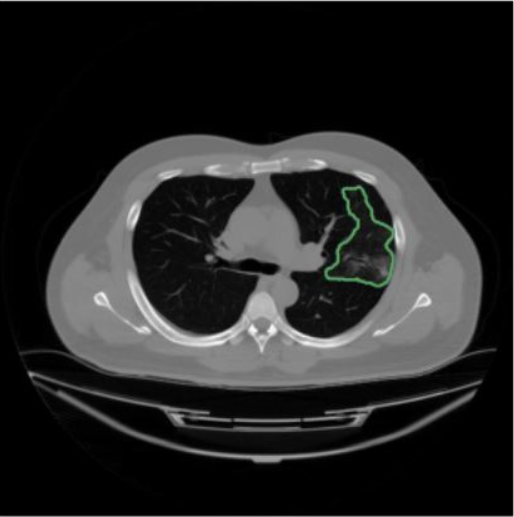
\includegraphics[width=0.45\columnwidth]{Dense_1.1.PNG} 
    &
    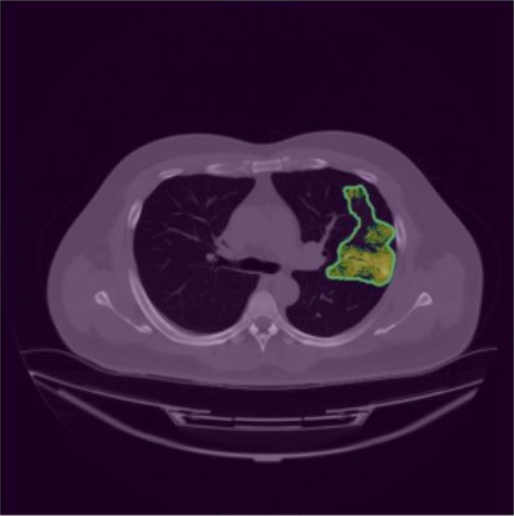
\includegraphics[width=0.45\columnwidth]{Dense_1.2.PNG} 
    \\
    (a) & (b)
    \end{tabular}
     \caption{Axial CT: inflammation mask (a) with original (expert) annotated boundary in green \cite{roth2021rapid}; (b) for (machine-identified/preprocessed) dense areas in yellow along with original boundary in green.}
     \label{Fig: Dense Masks}
\end{figure}
\end{comment}
\begin{figure*}
\centering
\begin{tabular}{c c c c}
    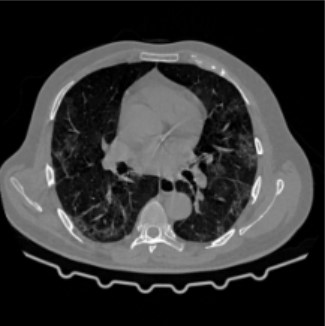
\includegraphics[scale=0.46]{Result1-30-ct.jpg} & \!\!
    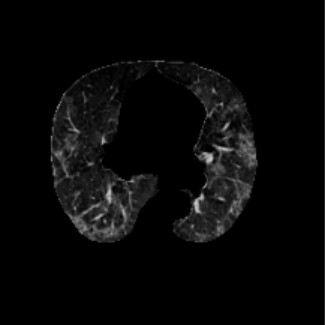
\includegraphics[scale=0.46]{images/Result1-30-extracted.jpg} & \!\!
    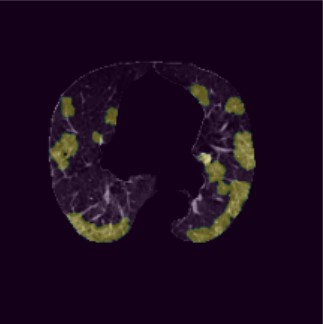
\includegraphics[scale=0.46]{images/Result1-30-unet.jpg} & \!\!
    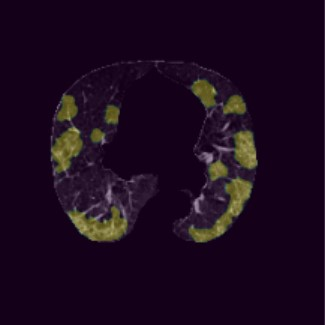
\includegraphics[scale=0.46]{images/Result1-30-capsnet.jpg}\\
    
    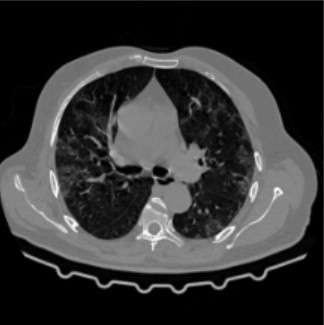
\includegraphics[scale=0.46]{images/Result2-25-ct.jpg} & \!\!
    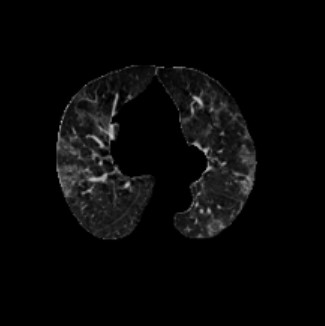
\includegraphics[scale=0.46]{images/Result2-25-extracted.jpg} & \!\!
    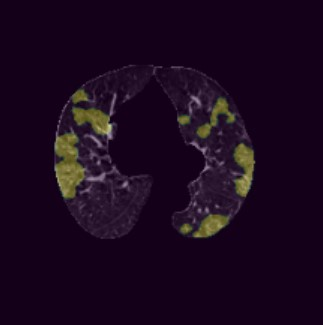
\includegraphics[scale=0.46]{images/Result2-25-unet.jpg} & \!\!
    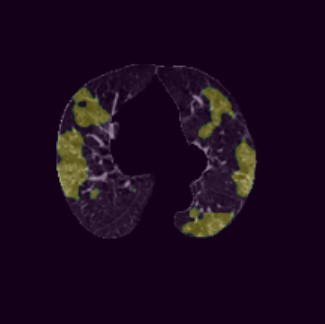
\includegraphics[scale=0.46]{images/Result2-25-capsnet.jpg}\\
    
    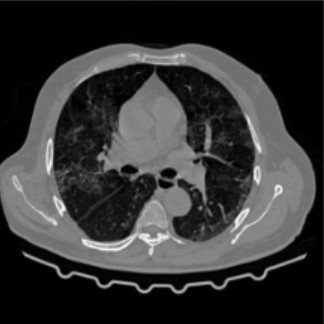
\includegraphics[scale=0.46]{images/Result3-27-ct.jpg} & \!\!
    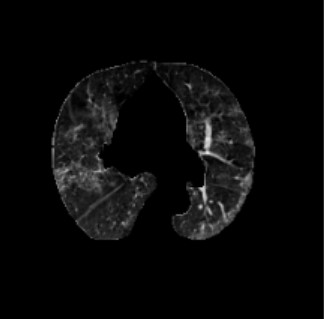
\includegraphics[scale=0.47]{images/Result3-27-extracted.jpg} & \!\!
    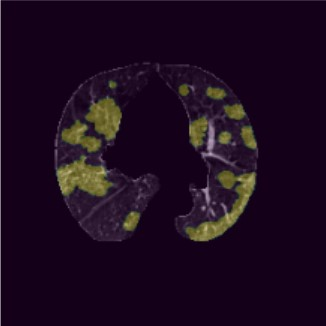
\includegraphics[scale=0.47]{images/Result3-27-unet.jpg} & \!\!
    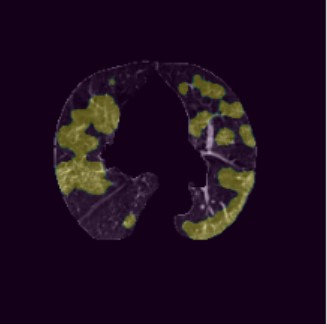
\includegraphics[scale=0.47]{images/Result3-27-capsnet.jpg}\\
    (a) & (b) & (c) & (d)
\end{tabular}
\caption{{(a)} Axial slice of CT scan; {(b)} Region Of Interest; {(c)} Inflammation Segmentation using UNet++; (d) Inflammation Segmentation using SegCaps.}
\label{Fig : Main Results}
\end{figure*}




\section{{Materials and Methods}}
\label{sec:MM}

Public datasets of chest CT scans of COVID-19 patients with annotated lung findings were used to train the deep networks UNet++ and SegCaps. A part of the study involving retrospective patient data was approved by the Institute Review Board (IRB) of Mahatma Gandhi Medical College and Hospital (MGMCH), Jaipur, India. The informed consent was waived due to the retrospective observational nature of the study and all data were anonymized before being analysed by research team, who were not part of the clinical team. All methods were performed in accordance with the relevant guidelines and regulations of the IRB of MGMCH.

\subsection{{Data Description}}
\label{sec:Data Description}
\begin{comment}
Of the COVID-19 CT Lung and Infection Segmentation Dataset \cite{jun2020covid}, we made use of a subset with 2581 non-contrast axial  CT scans (with both slice thickness and distance of 1-1.2mm) from 10 subjects for developing a lung segmentation model \cite{coronacases}.
\end{comment}
For training and testing inflammation segmentation models, we used the dataset from COVID-19 Lung CT Lesion Segmentation Challenge with 13705 non-contrast axial CT scans (with both slice thickness and distance of 5mm) from 199 subjects \cite{roth2021rapid}.
Clinical and radiological data of 302 subjects were collected at MGMCH. This dataset was used, for comparing the algorithmically quantified lung inflammation with the CT severity score manually obtained by the radiologist.
%Clinical and radiological data was collected at MGMCH between October to Decmeber 2020. This dataset was used, for comparing the algorithmically generated lung inflammation quantification with the manually calculated CT severity score by a radiologist. This dataset included CT scans as well as clinical, demographic, biochemical, and CT severity score for 302 COVID19 patients. Volumetric thin section CT scans were obtained with slices of 0.6mm each with high spatial frequency. This dataset also had missing values which was handled using data imputation. Mainly, the missing day of presentation was imputed with the median value. Remaining features which contained missing values were imputed using the nearest neighbors method with the assumption that data with similar values of known parameters may also have similar values for the unknown parameters.



\subsection{Segmentation Methods}
\label{sec:Segmentation Methods}

The task of semantically segmenting an image can be accomplished by designing a deep structure that extracts useful features using suitable arrangement of convolution operations, and summarizes such information to create a segmentation map as an output. Next, we describe UNet++ and SegCaps, the two such structures at hand.

\subsubsection{UNet++}

A predecessor CNN model, UNet, consists of encoder-decoder architecture with skip pathways connecting encoder blocks to decoder blocks. As depicted in Fig. \ref{fig:models}(a), UNet++ brings in three additions, namely, redesigned skip pathways, dense skip connections and deep supervision. These enable it to more effectively capture fine-grained details by gradually enriching high-resolution feature maps from the encoder network, and fusion with the corresponding semantically rich feature maps from the decoder network. While training this model, we performed the following augmentations: addition of Gaussian random noise with mean 0 and standard deviation 0.01, random rotations in the range -10 to 10 degrees, and random cropping to central 90\% of the image. The 1 - intersection over union (IOU loss) was minimized using was Adam optimizer with initial learning rate of $10^{-4}$.


\subsubsection{SegCaps}

In contrast to CNN models, which represent neuron-level information as scalars, capsule networks represent
such information as vectors of  spatial orientation, magnitude and other attributes. Specifically, we adopt the SegCaps architecture, consisting of various 2D convolution and deconvolution operations giving rise to 16D (16-dimensional) capsules,
and utilizing dynamic routing, as depicted in Fig. \ref{fig:models}(b). The SegCaps possesses 95.4\% fewer parameters compared to the UNet++. The same method was followed for training this models as that of UNet++ with the exception of removing rotation augmentation for this model.

%\subsection{Lung Segmentation}
%\label{sec:Lung Segmenation}



\subsection{Inflammation Segmentation}
\label{sec:Inflammation Segmenation}

Given a chest CT scan, we delineated the entire lung region by generating suitable lung mask as detailed elsewhere \cite{Sinha2022.01.30.22269998}, and used it as the region of interest (ROI). The original annotations of inflamed regions appear to often be overestimates. This can be seen in a representative case (Figs. \ref{Fig : Radiologist comparison}(a) and \ref{Fig : Radiologist comparison}(b)), where a practicing senior radiologist re-performed the annotation. Further, healthy lung areas being labeled as anomalous potentially confound ML models. To avoid this, we shrank the originally annotated region to a high-severity subregion using morphological geodesic active contour (Fig. \ref{Fig : Radiologist comparison}(c)) \cite{caselles1997geodesic}. Subsequently, we used such shrunk regions as baseline for training and testing our models. 

We measure segmentation accuracy in terms of Dice coefficient (DC) between predicted ($Y$) and baseline ($X$) inflammation regions, defined by $\mbox{DC} = {2|X\cap Y|}/{|X|+|Y|}$,
where $|X|$ indicates the area of $X$. By stacking, we also generated and quantified lung and inflammation volumes, and reported automated lesion to lung ratio (ALLR), the fraction of lung volume that is inflamed \cite{Sinha2022.01.30.22269998}.



\begin{comment}
Training segmentation models directly on the dataset resulted in poor performance in terms of dice score and one possible explanation is that the annotations for the Inflammation mask had both the regions having high and low density of abnormalities. Separating those two regions can improve the performance of the model. The dense region was computed by shrinking the annotations using morphological geodesic active contour, we used that dense region of abnormality as ground truth mask for further segmentation tasks as shown in Fig \ref{Fig: Dense Masks}.
\end{comment}

\begin{comment}
\\
    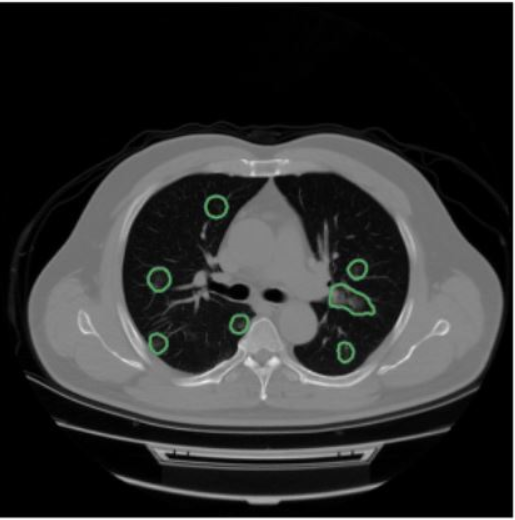
\includegraphics[width=0.45\columnwidth]{Dense_2.1.PNG} 
    &
    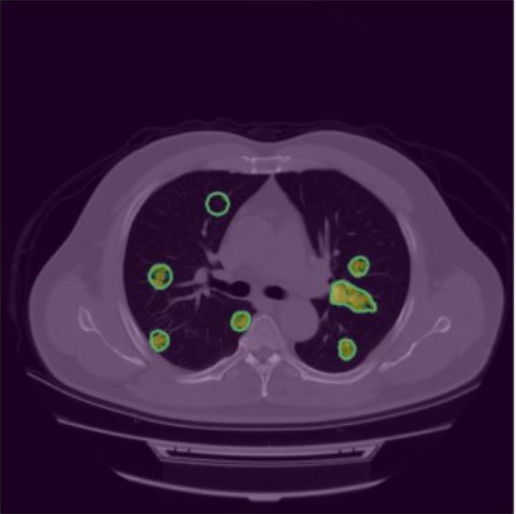
\includegraphics[width=0.45\columnwidth]{Dense_2.2.PNG} 
    \\
    (c) & (d)
\end{comment}

\begin{table}[t!]
    \centering
    \caption{Test Dice coefficient for inflammation segmentation using UNet++ and SegCaps}
    \begin{tabular}{ccc}
    \toprule 
        \textbf{Model} & \textbf{Number of epochs} & \textbf{Test Dice coefficient} \\ 
%        & \textbf{epochs} & \\
    \midrule
        UNet++ & 30 &  60\% \\
    %\hline
       SegCaps & 30 &  59.57\% \\
       \bottomrule
    %\hline 
    \end{tabular}
    \label{tab:2d-IS}
\end{table}


% UNet++ and SegCaps model were trained for binary segmentation of each of the classes.

%The following augmentations were applied to the input image and corresponding mask while training the UNet++ and SegCaps model: addition of gaussian random noise with mean 0 and standard deviation 0.01, random rotations in the range -10 to 10 degrees only in UNet++, random cropping to central 90\% of the image. The loss used was iou\_loss, and the optimizer used was Adam with initial learning rate of $10^{-4}$.

% The masks are calculated for each axial slice in a CT scan. These masks are then stacked to form a 3d Inflammation volume for a CT scan.


%as defined below:
%\begin{align*}
%\textit{ALLR} = \frac{\textit{Volume of the inflammation}}{\textit{Volume of the lung}}
%\end{align*}

% For a given CT scan first the lungs are segmented, then the inflammation region is segmented using the ROIs to calculate the ALLR. The segmentation of Inflammation region is based on the generated mask after pre-processing.

\subsection{Outcome Prediction}

Elsewhere, an ML model has been developed based on MGMCH dataset to predict an incoming COVID-19 patient's need for mechanical ventilation (MV) based on demographic, biochemical as well as the radiological parameters, and ALLR based on UNet++ and manual CT severity score have been found to perform comparably \cite{Sinha2022.01.30.22269998}. In this paper, we shall compare the performance of ALLRs based on UNet++ and SegCaps in terms of the area (AUC) under the median receiver operating characteristic (ROC) curve.


%ical as well as the radiological parameters based on the chest CT scan (if performed) along with the pre-existing conditions. For this task, we used the patient records to develop a machine learning model which predicts that whether there is a need for mechanical ventilation(MV), an acutely scarce resource, based on the MGMCH dataset. Prediction of such need is a clinically meaningful and significant outcome, which may guide efficient triaging (e.g., patients in need of MV should be admitted to a hospital in a unit where they can be monitored effectively). Now, whether patient need mechanical ventilation or not was posed as a classification task. And in order to do this task, we compared the performance with well known ensemble techniques and concluded that random forest is performing better as comparable to other models in terms of generalizability and robustness.

%The receiver operating characteristic(ROC) curve is plotted by calculating true positive rate (TPR) and false positive rate (FPR) for various threshold points of the probability generated by the model. ROC curve is convex by definition so we took the convex hull of the curve where the operating points between the optimal points are obtained by time sharing. We also calculated the area under the curve (AUC) to compare different segmentation models. It is a more useful performance metric than accuracy in cases of class imbalance, which is present in the MGMCH dataset.

